\documentclass{article}
\usepackage[usenames]{color} %used for font color
\usepackage{amssymb} %maths
\usepackage{amsmath} %maths
\usepackage{amsfonts}
\usepackage[utf8]{inputenc} %useful to type directly diacritic characters
\usepackage{soul}
\usepackage{bm}
\usepackage{graphicx}
\graphicspath{{./figures/}}                % 画像フォルダを宣言
\DeclareGraphicsExtensions{.pdf,.png,.jpg,.jpeg} % 候補拡張子

\def\x{\bm{x}}
\def\y{\bm{y}}
\def\c{\bm{c}}
\def\d{\bm{d}}
\def\A{\bm{A}}
\def\B{\bm{B}}
\def\b{\bm{b}}
\def\y{\bm{y}}
\def\Re{\mathbb{R}}
\def\Z{\mathbb{Z}}

\title{ISyE 6669 HW 1}
\date{Fall 2025}
\begin{document}
\maketitle


\begin{enumerate}
\item Consider the following maximization problem
\begin{align*}
    \max\quad & x^2 + (y-1)^2 \\
\text{s.t.}\quad & x + 2y \le 6 \\
& x - y \le 0 \\
& x \ge 0,\ y \ge 0.
\end{align*}
Plot the feasible region of this problem with the feasible area shaded. Draw (in dashed lines) the contours of the objective function. Based on your 
drawing, find all the optimal solutions and the optimal objective value of this problem. There may be multiple optimal solutions. Find all optimal solutions.

\hrulefill

\textbf{Solution.}


Looking at the six graphs in Figure 1, you can see a white triangular area in each plot. This white triangular region represents the set of points that satisfy all the constraints of the problem.

The problem is to maximize $x^2 + (y-1)^2$, and the black circles in the figures are the contours of this objective function. The contour values increase from left to right and top to bottom, corresponding to $x^2 + (y-1)^2 = 1$ up to $x^2 + (y-1)^2 = 6$.

Note that since $x^2 + (y-1)^2 \geq 0$ for all real $x, y$, the objective function cannot take negative values, so we only need to consider non-negative contour values.

As the contour value increases, the circles get larger and start to touch the white feasible area except the origin. At a contour value of 4, the circle is tangent to the feasible region at the point $(0, 3)$. When the contour value is 5, the circle is tangent at the point $(2, 2)$. For contour values greater than 5, the circles no longer intersect the feasible region.

Therefore, the maximum value of $x^2 + (y-1)^2$ over the feasible region is 5, and the optimal solution is at the point $(x, y) = (2, 2)$.







\begin{figure}[htbp]
    \centering
    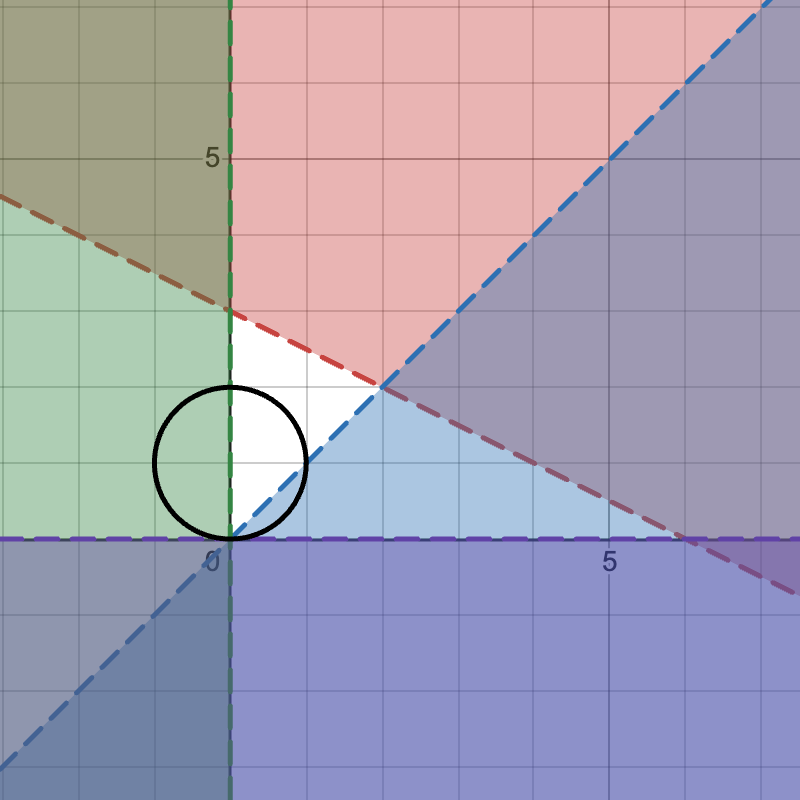
\includegraphics[width=0.45\textwidth]{figures/HW1_a-1.png}
    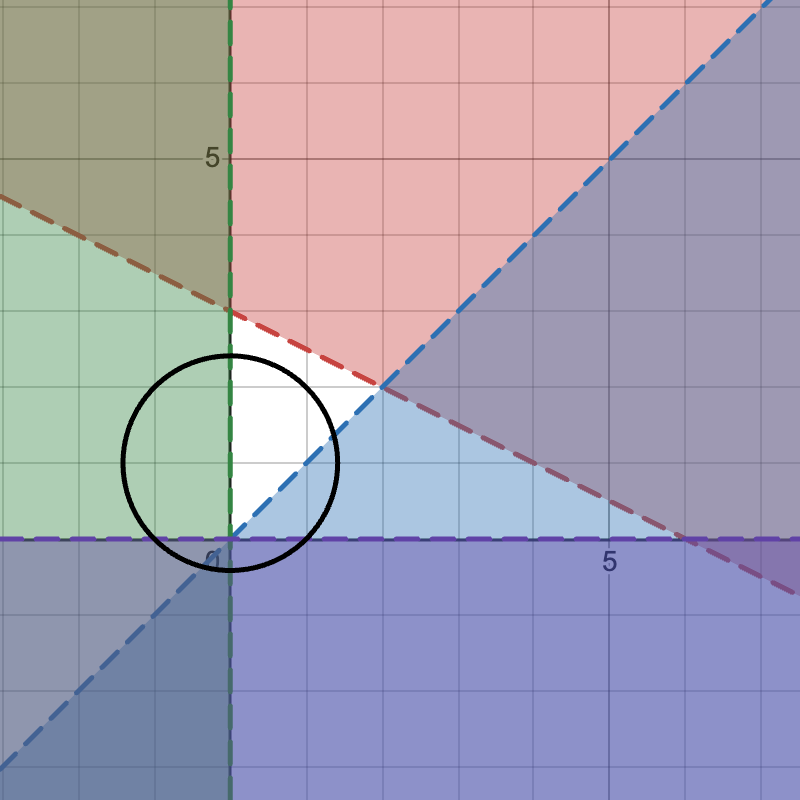
\includegraphics[width=0.45\textwidth]{figures/HW1_a-2.png}
    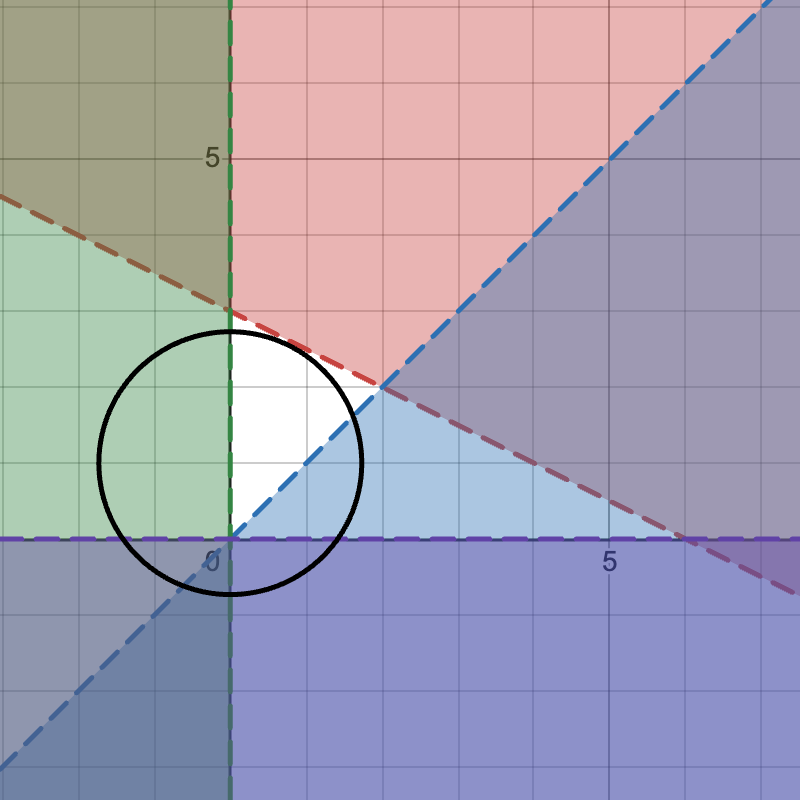
\includegraphics[width=0.45\textwidth]{figures/HW1_a-3.png}
    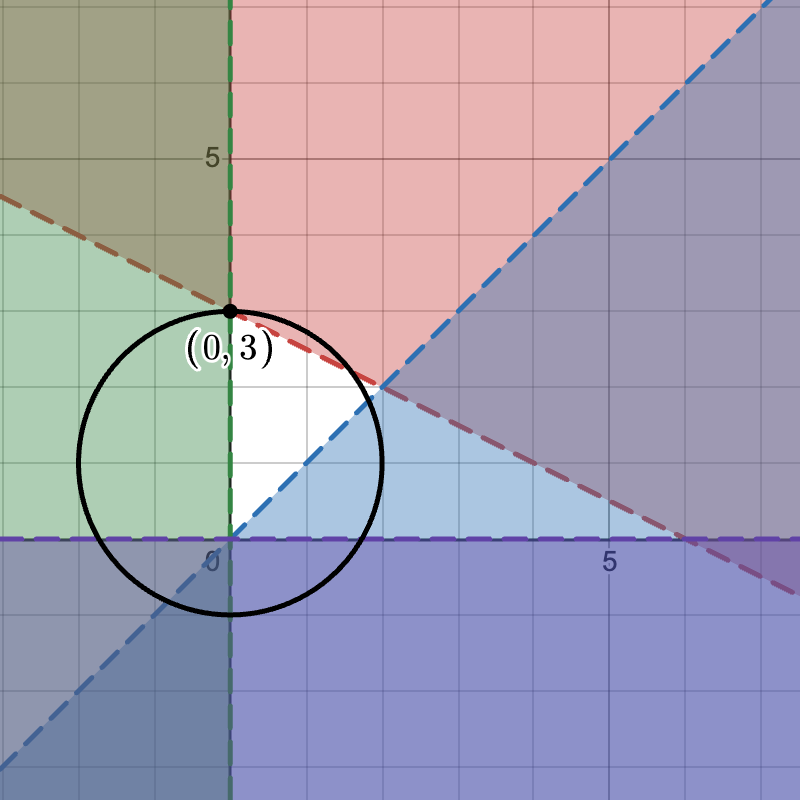
\includegraphics[width=0.45\textwidth]{figures/HW1_a-4.png}
    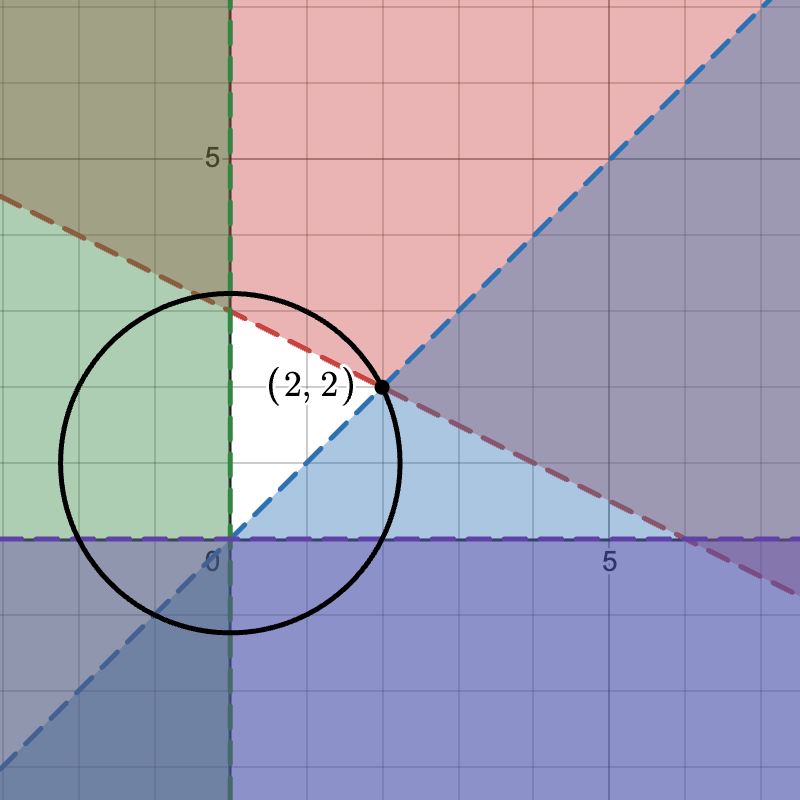
\includegraphics[width=0.45\textwidth]{figures/HW1_a-5.png}
    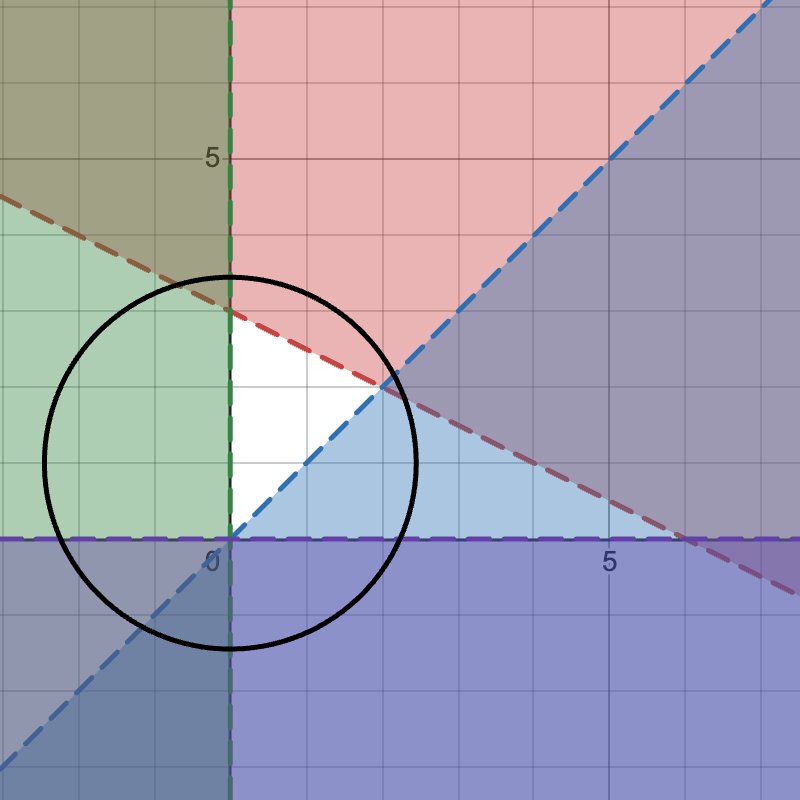
\includegraphics[width=0.45\textwidth]{figures/HW1_a-6.png}
    \caption{Feasible region and objective contours for various $x^2 + (y - 1)^2$ values ($x^2 + (y - 1)^2 = 1$ to $x^2 + (y - 1)^2 = 6$).}
    \label{fig:hw1_a1to6}
\end{figure}



\item Solve the following problem using basic calculus:
$$\max\{ -10x + 5x^{2\ }+9x^{3}+\ 8x^{4}+7x^{5}:  \ -1 \le x \le 1\}$$
What is the optimal solution and the optimal objective value? Are there any local maxima that are not global maxima? 


\hrulefill

\textbf{Solution.}

\medskip
\underline{Step 1. First derivative and critical points}

\[
f'(x) = 35x^4 + 32x^3 + 27x^2 + 10x - 10.
\]
This is a quartic equation, which is difficult to solve exactly.  
However, we can analyze the number and location of critical points using sign checks and convexity.

\medskip
\underline{Step 2. Convexity of $f'$}

The second derivative is:
\[
f''(x) = 140x^3 + 96x^2 + 54x + 10,
\]
and the third derivative is:
\[
f'''(x) = 420x^2 + 192x + 54.
\]
Since the discriminant of $f'''(x)$ is negative, $f'''(x) > 0$ for all real $x$.  
Therefore, $f''(x)$ is strictly increasing, which implies that $f'(x)$ is a \emph{strictly convex} function.  
A strictly convex quartic can have at most two real roots.

\medskip
\underline{Step 3. Sign checks to locate roots}

We evaluate $f'(x)$ at several points:

\[
\begin{aligned}
f'(-1) &= 10 > 0, \\
f'(0) &= -10 < 0, \\
f'(1) &= 94 > 0.
\end{aligned}
\]
Since $f'(x)$ is convex and changes sign, there must be exactly two real roots: one in $(-1,0)$ and one in $(0,1)$.  
Using additional test points:
\[
f'(-0.9) \approx 2.5 > 0, \quad f'(-0.85) \approx -0.37 < 0,
\]
so the left root lies in $(-0.875, -0.85)$.  
Similarly:
\[
f'(0.375) \approx -0.07 < 0,\quad f'(0.4) \approx 1.26 > 0,
\]
so the right root lies in $(0.375, 0.4)$.

\medskip
\underline{Step 4. Increasing/decreasing intervals}

From the sign of $f'$:

- Increasing on $[-1, \, x_1)$ where $x_1 \approx -0.86$,
- Decreasing on $(x_1, \, x_2)$ where $x_2 \approx 0.38$,
- Increasing again on $(x_2, \, 1]$.

Thus, $x_1$ is a local maximum, $x_2$ is a local minimum.

\medskip
\underline{Step 5. Compare function values}

We check $f(x)$ at candidate points:

\[
\begin{aligned}
f(-1) &= 7, \\
f(1) &= 19, \\
f(0) &= 0.
\end{aligned}
\]
Near the left local maximum ($x \approx -0.86$),  
\[
f(-0.85) \approx 7.66.
\]
Therefore, the local maximum value is about $7.66$, which is \emph{less} than $f(1)=19$.

\medskip
\underline{Step 6. Final answer}

- The \textbf{optimal solution} is:
\[
x^\ast = 1.
\]
- The \textbf{optimal objective value} is:
\[
f(x^\ast) = 19.
\]
- There exists a \textbf{local maximum} at $x \approx -0.86$, but it is not a global maximum.

\hrulefill

\textbf{Summary Table:}

\[
\begin{array}{c|cccccc}
x & -1 & \cdots & x_1 & \cdots & x_2 & \cdots 1 \\ \hline
f'(x) & + & & 0 & & 0 & + \\
f(x) & \nearrow & \ \ \max\ \  & \searrow & \ \ \min\ \  & \nearrow &
\end{array}
\]


\item Consider the following optimization problem:
\begin{align*}
    (P)\quad \max \quad & x (z^2 - y^2) \\
    \text{s.t.}\quad & y + |z|\le 1, \\
    & x \in \{0,1\}, \; y\ge 0.
\end{align*}
Answer the questions:
\begin{enumerate}
    \item Is (P) a linear program, a mixed integer nonlinear program, or a mixed integer quadratic program? Choose all descriptions that apply.
    
    \item Write a minimization problem that is equivalent to (P).
    
    \item Find all the optimal solutions.
\end{enumerate}

\hrulefill

\textbf{Solution.}
\begin{enumerate}
    \item[(a)] (P) is a \textbf{Mixed Integer Nonlinear Program} (MINLP).

    \begin{itemize}
        \item The objective function $x(z^2 - y^2)$ is nonlinear because $x$ is an integer variable ($0$ or $1$), $y$ and $z$ are continuous variables, and the terms $z^2$ and $y^2$ are quadratic.
        \item The constraint $y + |z| \le 1$ is also nonlinear due to the absolute value $|z|$.
        \item Therefore, (P) is classified as a \textbf{Mixed Integer Nonlinear Program (MINLP)}.
        \item Although the objective function is quadratic, the presence of $|z|$ means it is \emph{not} a Mixed Integer Quadratic Program (MIQP).
        \item It is also not a Linear Program (LP).
    \end{itemize}

    \item[(b)] An equivalent minimization problem to (P) can be written by minimizing the negative of the objective function:
    \begin{align*}
        -\min \quad & -x(z^2 - y^2) \\
        \text{s.t.}\quad & y + |z| \le 1, \\
        & x \in \{0,1\},\; y \ge 0.
    \end{align*}
    If the minimum value is $-v^\ast$, then the maximum value of the original problem (P) is $v^\ast$.

\begin{figure}[htbp]
    \centering
    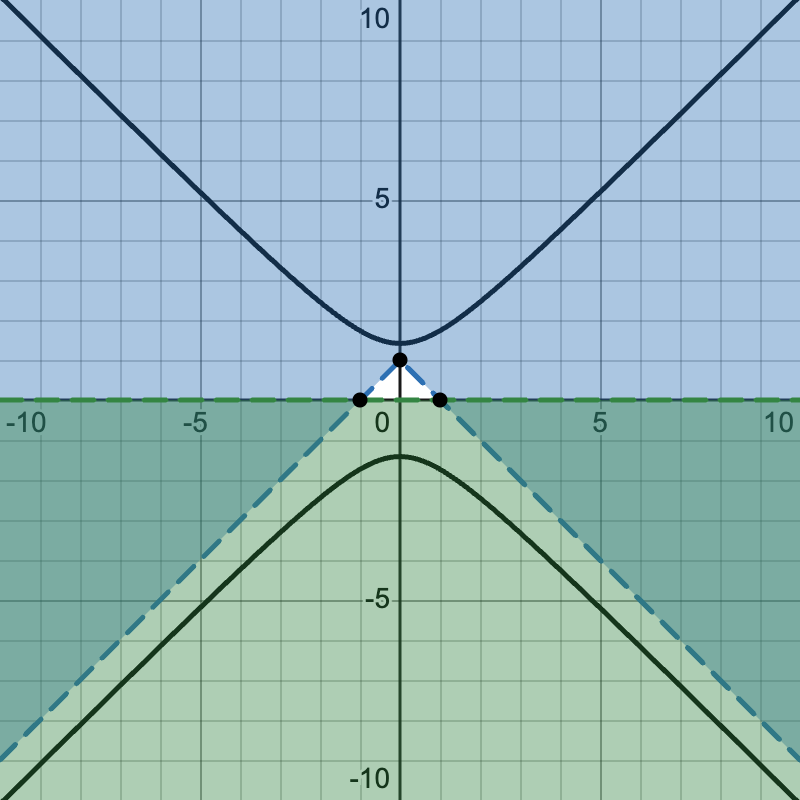
\includegraphics[width=0.45\textwidth]{figures/HW1_3_a_-2.png}
    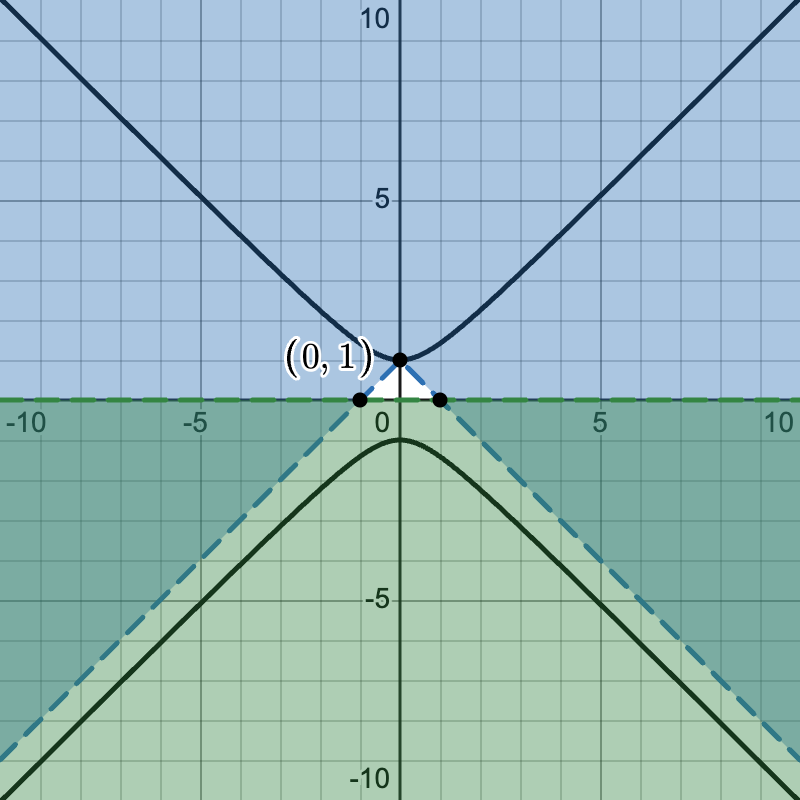
\includegraphics[width=0.45\textwidth]{figures/HW1_3_a_-1.png}
    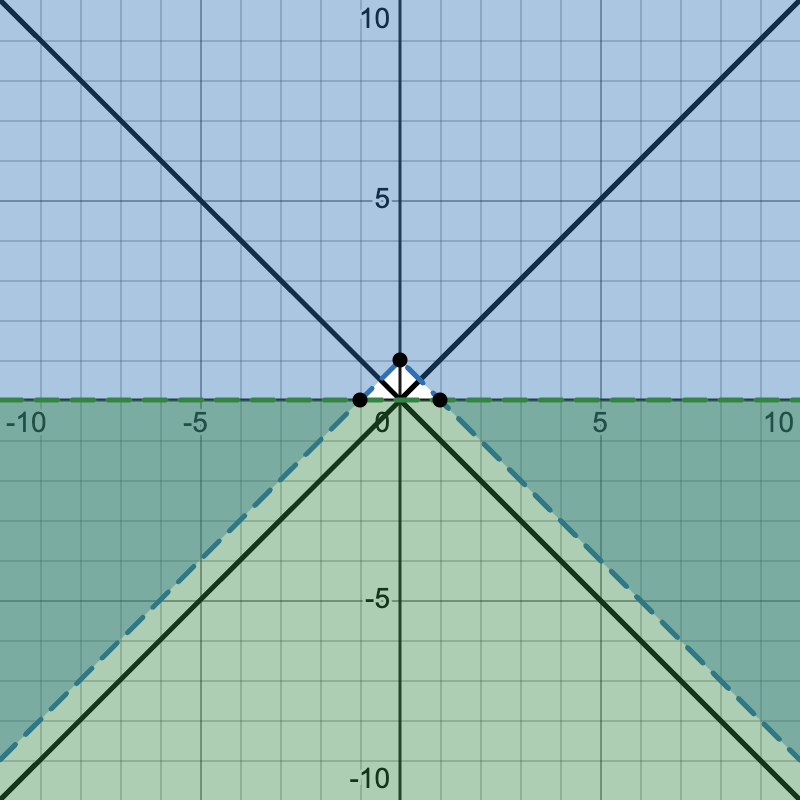
\includegraphics[width=0.45\textwidth]{figures/HW1_3_a_0.png}
    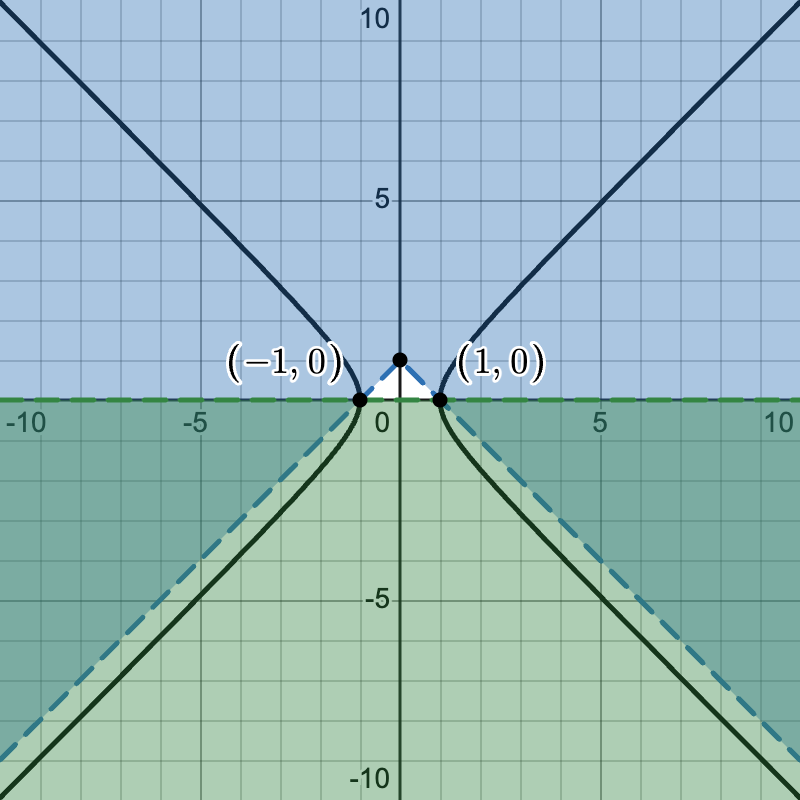
\includegraphics[width=0.45\textwidth]{figures/HW1_3_a_1.png}
    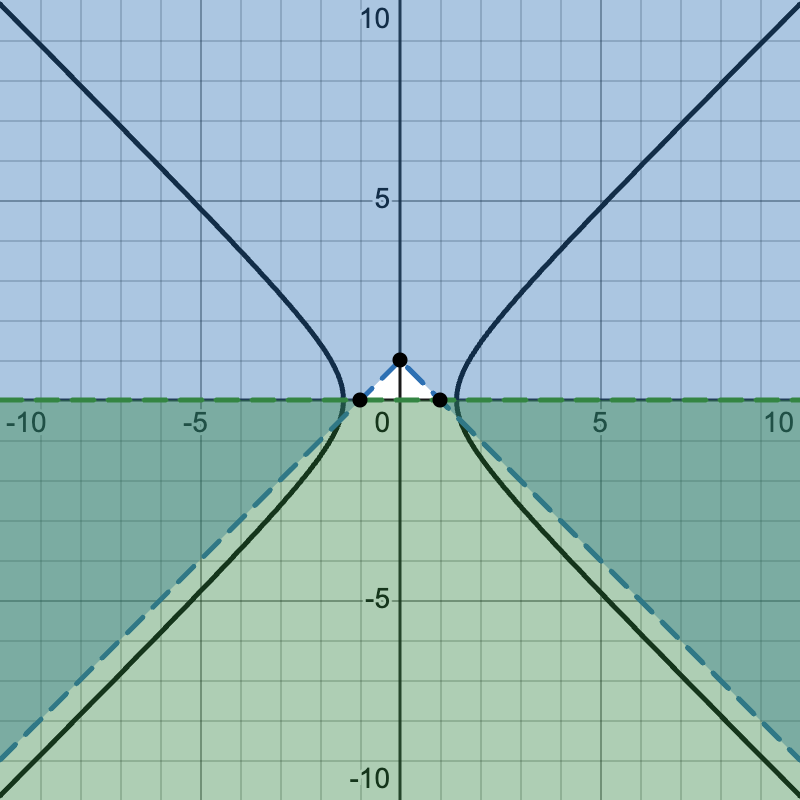
\includegraphics[width=0.45\textwidth]{figures/HW1_3_a_2.png}
    \caption{Feasible region and objective function contours for Problem 3. The white region represents the feasible set $y + |z| \le 1$, $y \ge 0$, and the colored contours show different values of the objective function $x(z^2 - y^2)$.}
    \label{fig:hw1_3_a}
\end{figure}

    \item[(c)] See Figure~\ref{fig:hw1_3_a} below. This figure shows the contour lines of the objective function $x(z^2 - y^2)$ for different values, and the white region represents the feasible set defined by $y + |z| \le 1$, $y \ge 0$.

    From the figure, we can observe the behavior of the objective function contours. When the objective value is less than $-2$, the contours do not intersect the feasible region. At $-1$, the contour first touches the feasible region. As the objective value increases, the contour for $1$ also touches the feasible region, but for $2$ and above, the contours again do not intersect the feasible region.

    Therefore, the maximum value of (P) is $1$.

    In this case, the optimal solutions are $x=1$, $y=0$, $z=1$ or $z=-1$. That is,
    \[
        (x^\ast, y^\ast, z^\ast) = (1, 0, 1) \quad \text{or} \quad (1, 0, -1)
    \]
    are the optimal solutions.

    To verify this is indeed optimal, we need to consider both cases for $x$:
    \begin{itemize}
        \item When $x=0$: The objective function $x(z^2 - y^2)$ is always $0$ regardless of the values of $y$ and $z$.
        \item When $x=1$: The objective function becomes $z^2 - y^2$, and from our analysis above, the maximum value achievable is $1$ at the points $(1, 0, 1)$ and $(1, 0, -1)$.
    \end{itemize}
    Since $1 > 0$, the optimal solution occurs when $x=1$, and the maximum value of (P) is $1$.

See Figure~\ref{fig:hw1_3_a} for visualizations of the feasible region and objective contours for various parameter values.

\end{enumerate}

\item Recall the portfolio optimization problem solved in Module 2, Lesson 3. Use the provided code file (\texttt{portopt\_cvxpy\_python3\_HW1.py}) and the provided data file (\texttt{monthly\_prices\_HW1.csv}) to solve the same portfolio problem with this new data. Compare and discuss the differences and similarities between this new solution and the one obtained in the lesson.

\hrulefill

\textbf{Solution.}

Using the provided data file \texttt{monthly\_prices\_HW1.csv} and running the code from \texttt{portopt\_cvxpy\_python3\_HW1.py}, we obtain the following results:

\begin{verbatim}
---------------------
MSFT: Exp ret = 0.024328, Risk = 0.062160
V: Exp ret = 0.019058, Risk = 0.040485
WMT: Exp ret = 0.030167, Risk = 0.056756
----------------------
Optimal portfolio
----------------------
x[MSFT] = 0.217181
x[V] = 0.581434
x[WMT] = 0.201385
----------------------
Exp ret = 0.022440
risk    = 0.034429
----------------------

The optimal portfolio in the lesson video (Module 2, Lesson 3 example) is as follows:
----------------------
MSFT: Exp ret = 0.024611, Risk = 0.058040
V: Exp ret = 0.018237, Risk = 0.042807
WMT: Exp ret = 0.009066, Risk = 0.044461
----------------------
Optimal portfolio
----------------------
x[MSFT] = 0.5828
x[V] = 0.2043
x[WMT] = 0.2129
----------------------
Exp ret = 0.020000
risk    = 0.038300
----------------------

\end{verbatim}

\textbf{Comparison:}

\begin{itemize}
    \item \textbf{Differences in Investment Allocation} \\
    In the lesson, the optimal investment allocation was MSFT: \$582.8, V: \$204.3, WMT: \$212.9 (for \$1000 investment), which represents MSFT: 58.3\%, V: 20.4\%, WMT: 21.3\%. With the new data, we have MSFT: 21.7\%, V: 58.1\%, WMT: 20.1\%. The investment allocation in V (Visa) has significantly increased, while MSFT (Microsoft) allocation has decreased substantially. WMT (Walmart) remains approximately the same.
    
    \item \textbf{Differences in Expected Return and Risk} \\
    In the lesson, the expected monthly return was \$20 (2.0\%) with risk (standard deviation) of \$38.3 (3.83\%). With the new data, the expected return is 2.24\% and risk is 3.44\%, showing a slight increase in return and decrease in risk.
    
    \item \textbf{Differences in Asset Risk (Standard Deviation)} \\
    Based on the new data, V (Visa) has the lowest risk (standard deviation of 0.0405) among the three assets, which leads to a higher allocation to V in the optimal portfolio. The allocation to MSFT (Microsoft) decreases, while WMT (Walmart) remains similar. This shift in allocation can be explained by the differences in the individual risks (standard deviations) of the assets as observed in the data, without referring to the covariance values.
    
\end{itemize}

\textbf{Summary:}

With the new data, V (Visa) has lower risk while maintaining sufficient return, leading to a significant increase in V allocation and decrease in MSFT allocation. Overall, the expected return has slightly increased while risk has slightly decreased. This demonstrates that the optimal portfolio adapts flexibly to changes in the underlying data.

\end{enumerate}

\end{document}